\section{Simulation Analysis }
\label{sec:simulation}

\subsection{AC/DC converter graphs}

In this section we evaluated the AC/DC converter proposed. To simplify the calculations for NGSpice, we have decided to use the circuit \ref{fig:Circuit_Base_S}, since using the ideal model for the transformer was causing NGSpice to slow down significantly.
In order to analise the circuit after the transiant period, we have chosen $t \in \left[ 10 ; 200 \right[ $ ms.

The graphs for NGSpice are displayed here, alongside the table with the required elements:

\begin{figure}[h] \centering
\vspace{-3cm}
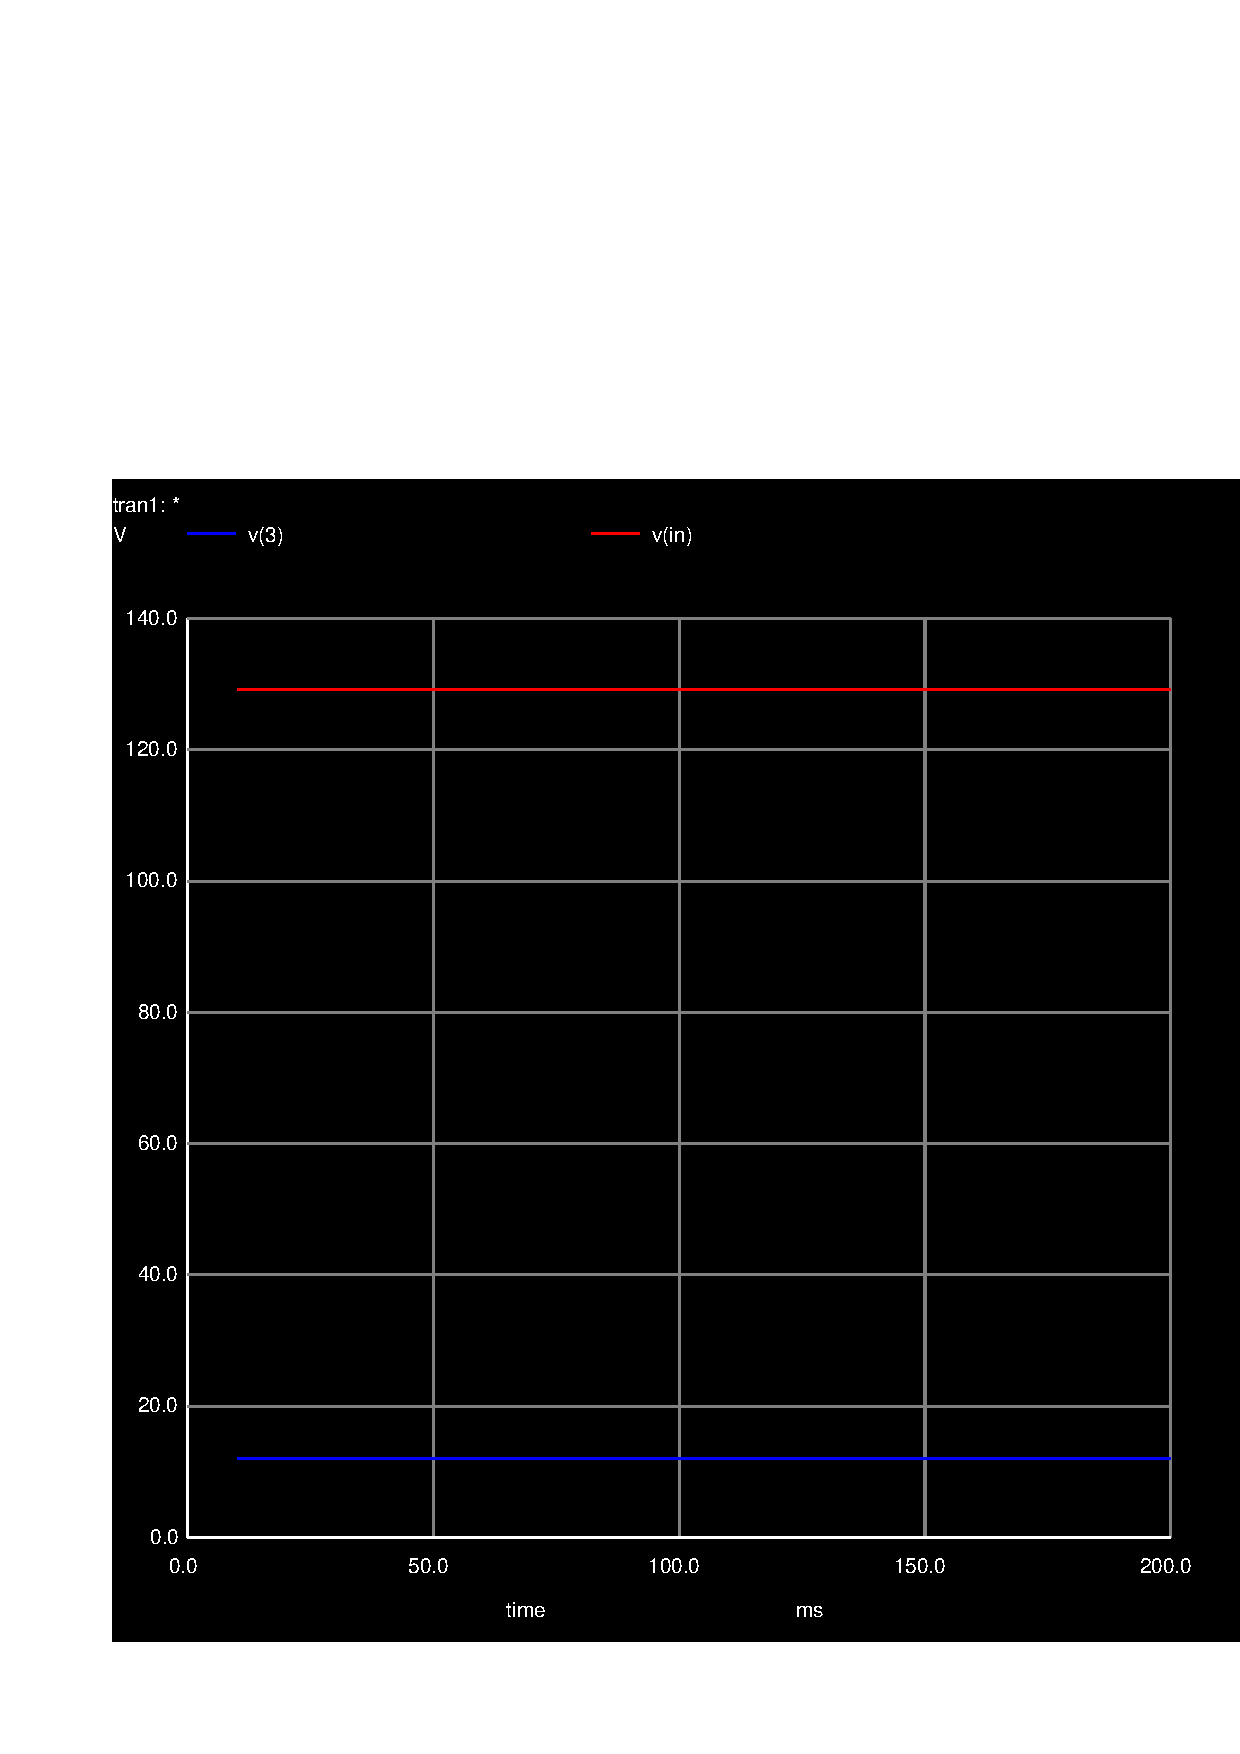
\includegraphics[height=11cm]{../sim/trans4.pdf}
\caption{$v_3(t)$ ($v_{OUT}(t)$) and $v_{IN}$ ($v_{Envelope}(t)$)}
\label{fig:SIM_FULL_RES}
\end{figure}

\begin{figure}[h] \centering
\vspace{-3cm}
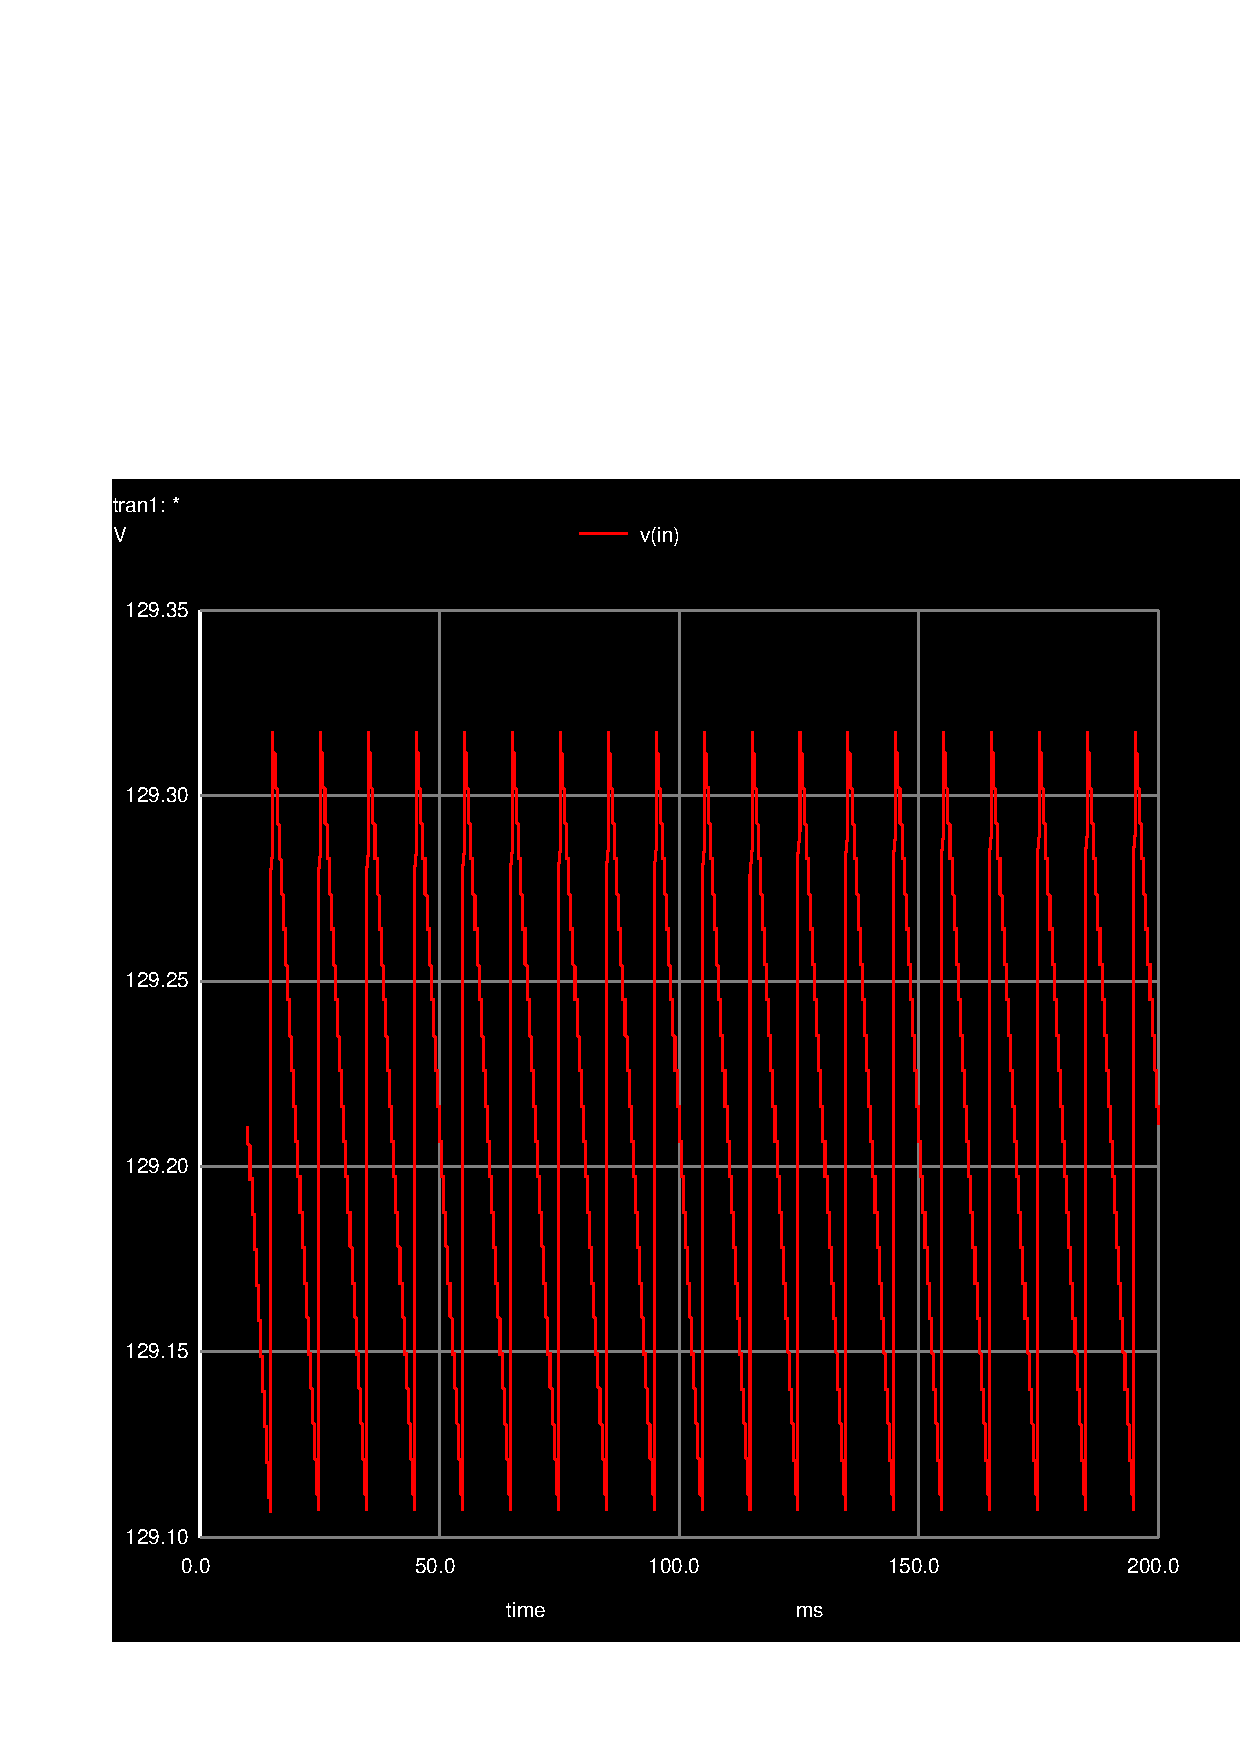
\includegraphics[height=11cm]{../sim/trans41.pdf}
\caption{$v_{IN}(t)$ ($v_{Envelope}(t)$)}
\label{fig:SIM_ENV}
\end{figure}

\newpage

\begin{figure}[h] \centering
\vspace{-3cm}
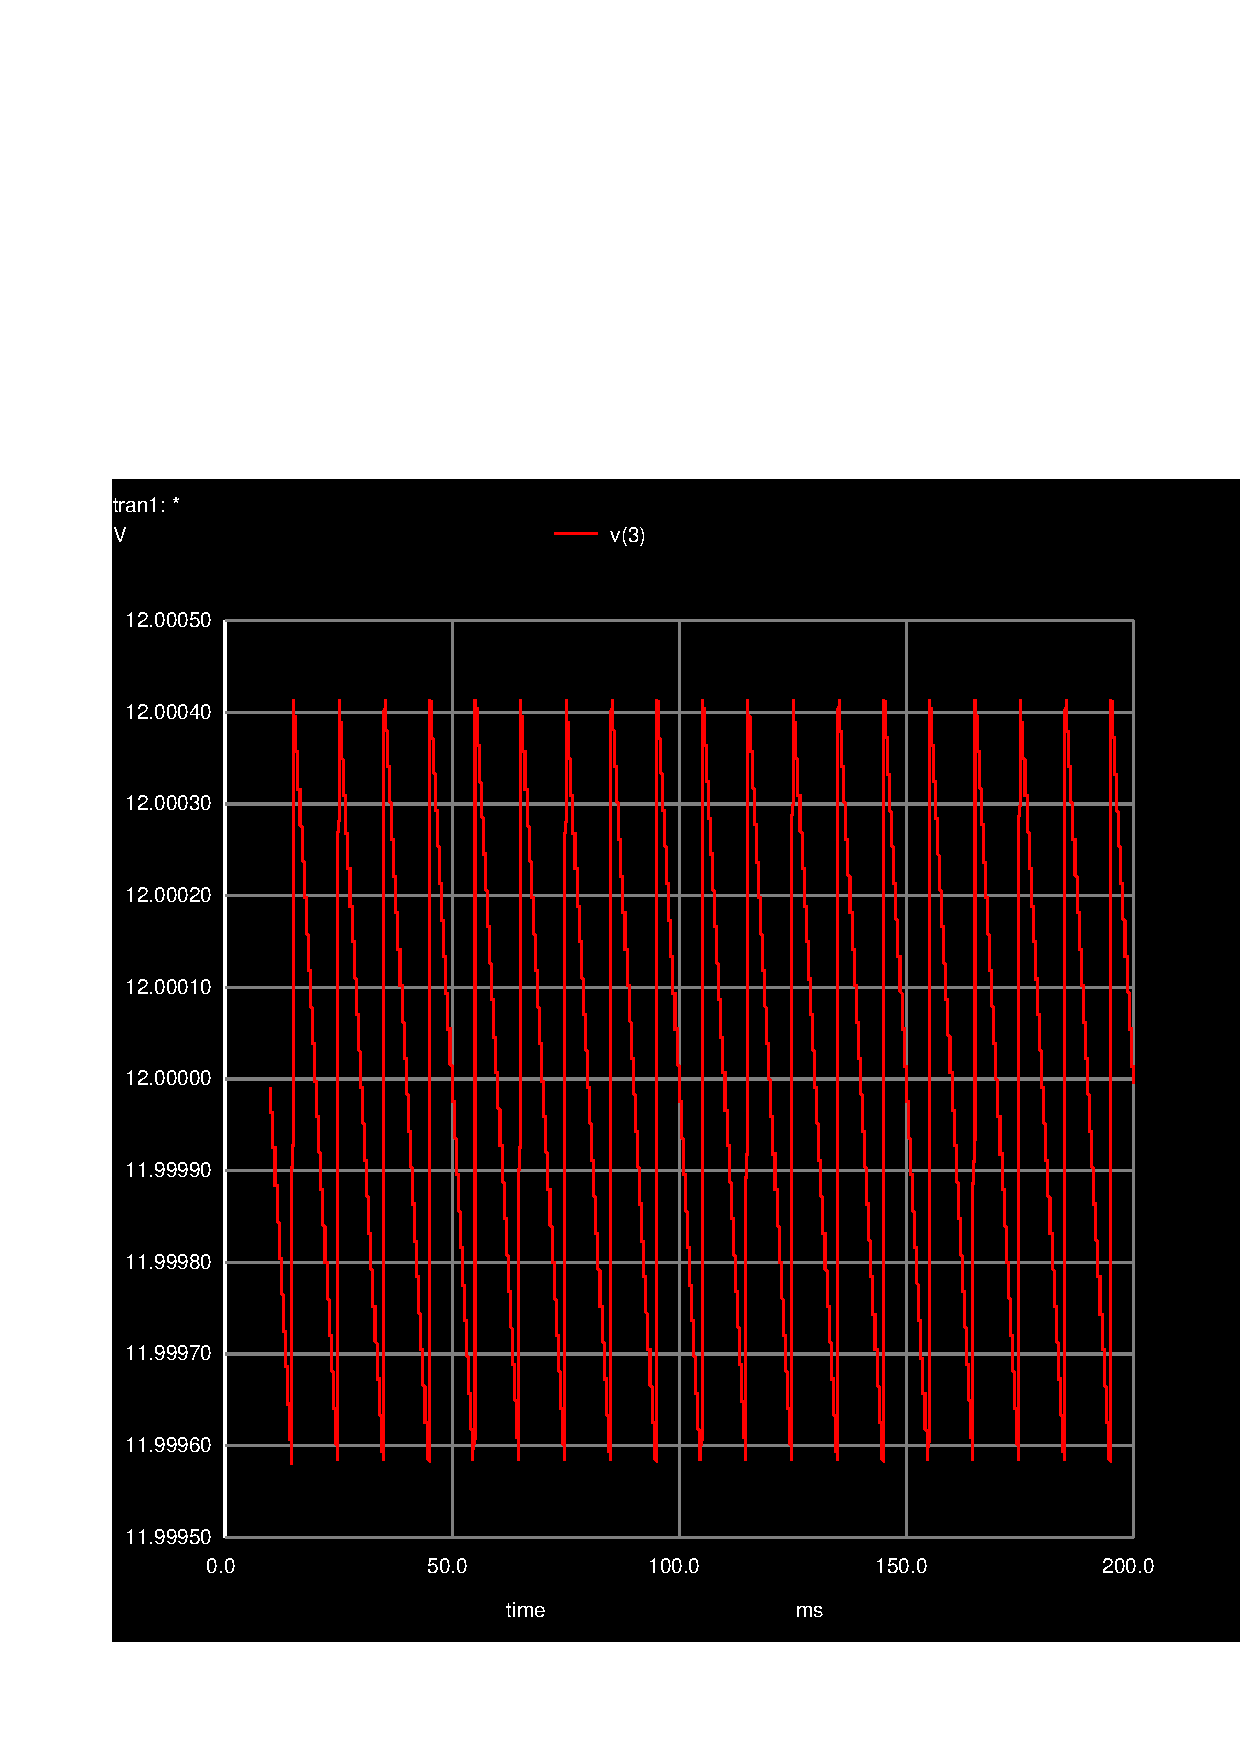
\includegraphics[height=11cm]{../sim/trans42.pdf}
\caption{$v_{3}(t)$ ($v_{OUT}(t)$)}
\label{fig:SIM_OUT}
\end{figure}

\begin{figure}[h] \centering
\vspace{-3cm}
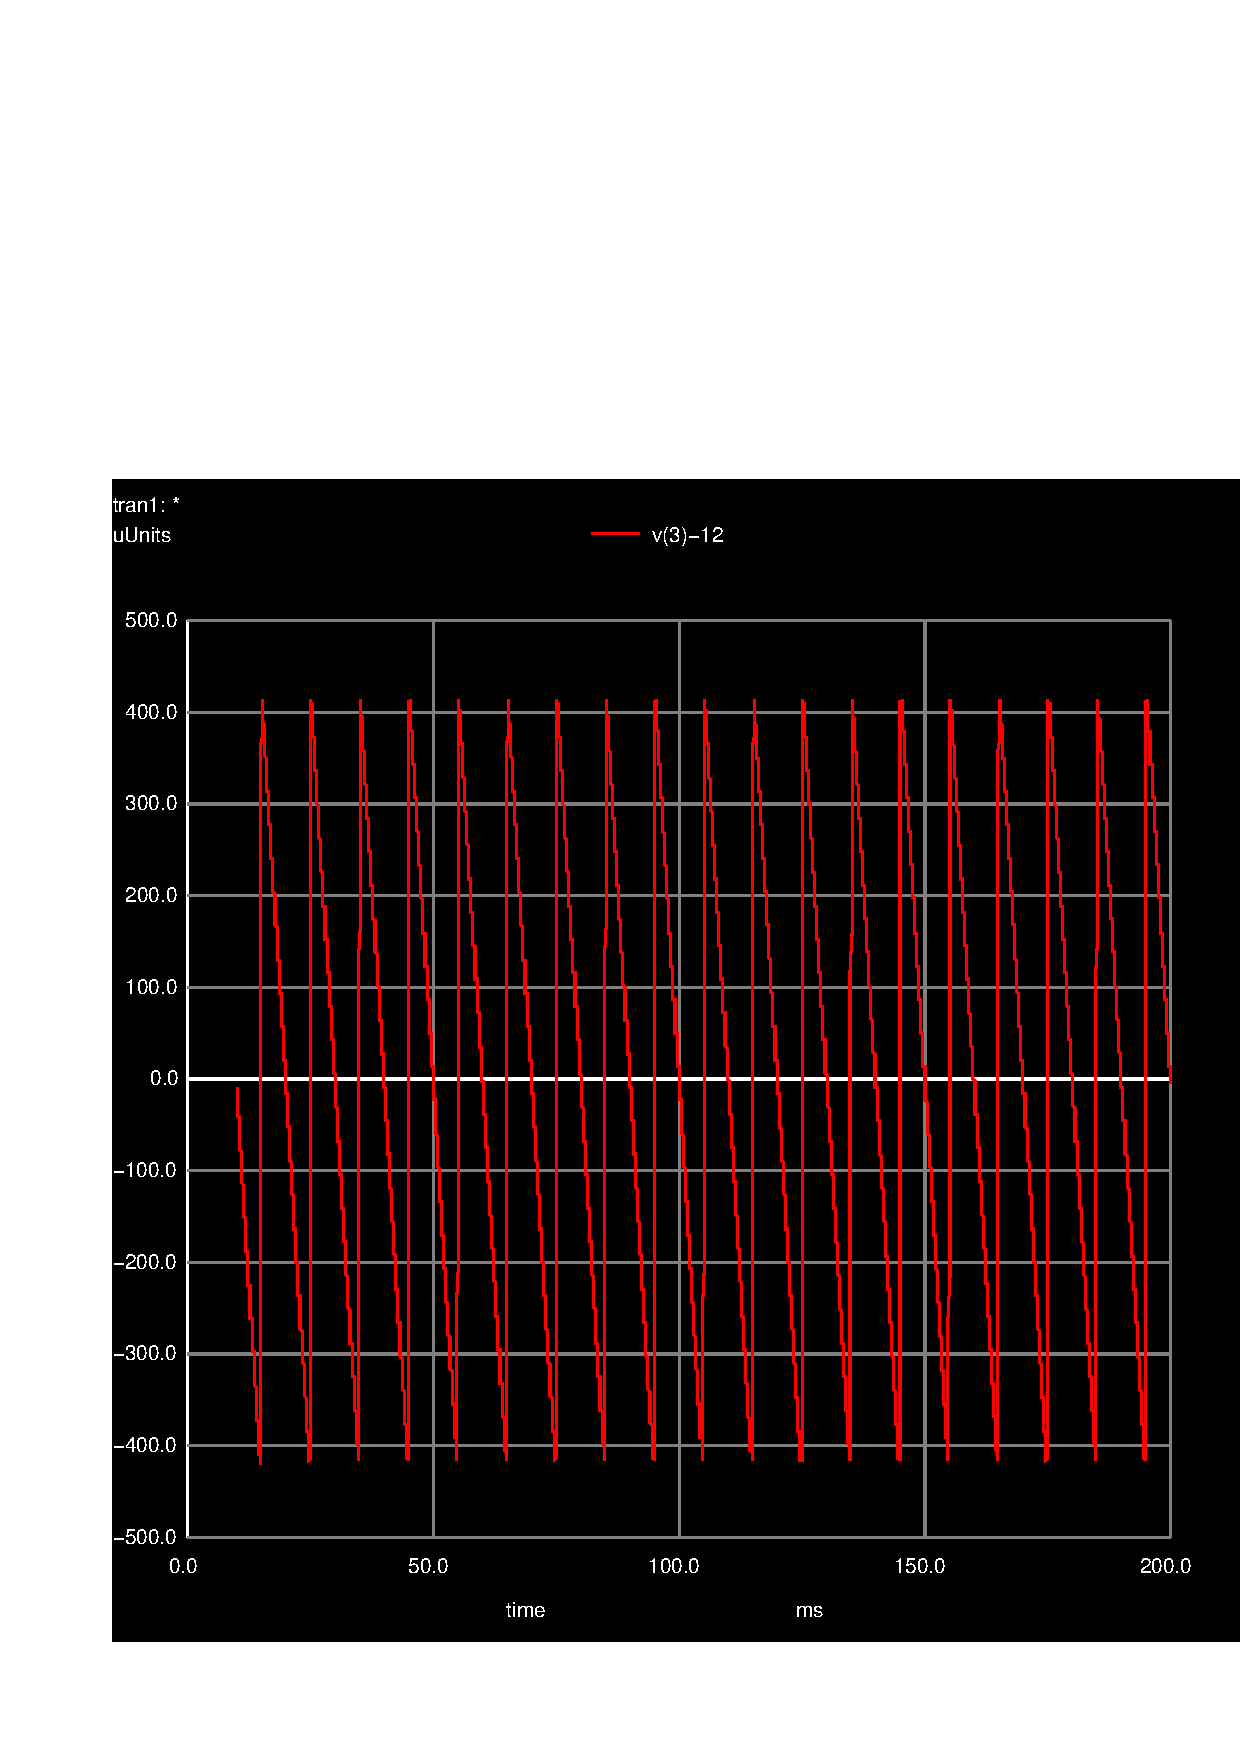
\includegraphics[height=11cm]{../sim/trans5.pdf}
\caption{$v_{3}(t)-12$ ($v_{out}(t)-12$)}
\label{fig:SIM_OUT-12}
\end{figure}

\newpage

Table~\ref{tab:SIM_RESULTADOS} shows the simulated operating point results for the circuit under analysis.
%Colocar a tabela 
\begin{table}[h]
  \centering
  \begin{tabular}{|l|r|}
    \hline    
    {\bf Name} & {\bf Value} \\ \hline
    n & 0.56882248\\ \hline
cost & 302.2\\ \hline
mean(v(3))-12 & 5.094465e-07\\ \hline
vecmax(v(3))-vecmin(v(3)) & 8.328428e-04\\ \hline
1 / (abs(mean(v(3))-12) + vecmax(v(3))-vecmin(v(3)) + 1u) / (150+150+(18 + 4)*.1) & 3.966031e+00\\ \hline

  \end{tabular}
  \caption{Merit is in {\it per voltage per cost} and expressed in Volt$^{-1}$UC$^{-1}$; other variables are of type {\it voltage} and expressed in Volt.}
  \label{tab:SIM_RESULTADOS}
\end{table}



